%!TEX root = ../thesis.tex
\chapter{Introduction}
\label{chapter_introduction}

When attempting to accomplish unfamiliar, complicated tasks, people often search for online tutorials to follow instructions. From using software applications, performing physical tasks such as cooking and assembling a machine, to free-form activities like sports and dance performance, each domain involves specific ``how-to'' knowledge with a certain degree of complexity \cite{ryle1945knowhow}.
%
However, producing high-quality instructions that are easy to follow requires authoring expertise and a significant time investment in editing practices from multimedia materials \cite{Muller:2009tw}. On the other hand, navigating a well-produced tutorial using existing tools remains inefficient for following step-by-step instructions.

In this dissertation, I present video-based computational approaches that enhance tutorial creation and consumption from author demonstrations. I encode the current practices from professional authors into automatic algorithms and interactive techniques.
%
My goal is to dramatically increase the quality of amateur-produced video instructions, which in turn improves learning for viewers who interactively navigate the content. I will introduce a set of interactive systems that cover both software applications (e.g., image manipulation tasks or browser navigation) and physical activities (e.g., Do-It-Yourself projects or dance movements) for recording, editing, and replaying instructional content.

% ---------------------------------------------------------------

\section{Challenges of Creating and Consuming Instructions}

Instructions, which contain the know-how and can be presented in different formats, enable novices to learn the domain knowledge and execute in action. The availability of content sharing sites such as YouTube\footnote{https://www.youtube.com/} and Instructables\footnote{http://www.instructables.com/} has enabled experts and hobbyists to create tutorials for a wide spectrum of topics \cite{Lafreniere:2012tl}. Among all the online support, videos are commonly used to present instructions. We suspect that users prefer videos over other formats for the following reasons:

First, consumer devices and software have become affordable for people to quickly record activities and later share via online platforms at minimum cost.
%
% ** describe the difficulties of making knowledge "explicit", esp. for actions and motions
Second, videos can be an efficient medium to document activities. Transferring know-how concisely and effectively to the audience is challenging. It especially requires efforts when a task involves \emph{tacit knowledge}, which is a kind of knowledge that is difficult to articulate in a written or verbal form \cite{polanyi1958personal, Klemmer:2006:BMF:1142405.1142429}. Examples of tacit knowledge include dancing, riding a bike, or driving nails with a hammer. Dancers can perform movements fluently with music. If they are asked to focus on the composite pieces, such as the arm and foot actions or rhythm, they might get confused and fail to express the entire movement. Very often, recording a video eases the difficulties of describing the entire activities in an explicit form.
%
This leads to another motivation that videos also provide an effective channel to convey ideas with adequate amounts of details. Learners can visually observe the exact actions in a video as if an expert were coaching in person.

However, while videos are easy to produce, they can include a lot of unnecessary footage. Inevitable content such as pauses, mistakes, and long repetitive actions makes it difficult for learners to focus on the most important steps and actions. A lot of authoring effort commonly goes into extracting footage, applying visual effects, and adding subtitles and annotations. On the other hand, given a well-edited video, navigating using a conventional video player remains inefficient. Learners with various needs could have a hard time skimming to an interesting moment or perceiving high-level overviews. Therefore, some prefer to follow static step-by-step tutorials, which are easy to scan forward and backward as instructions are listed in text and images. Similarly, it is time- and labor-intensive to produce this type of instructions, and can be limited in presenting complicated tasks.

% The goal of this dissertation to develop video-based recording, editing, and playback tools are optimized for creating and consuming instructional demonstrations. I combine the advantage of ubiquitous video recording with the benefits of video and structured tutorial formats. I aim to dramatically increase the quality of amateur-produced video instructions, which in turn improves learning for viewers who interactively navigate the content.

% ----- MixT ----- %

\subsection{New Tutorial Formats}

Both static and video tutorials have strengths, but my study showed that neither format is well suited for followers with various learning needs.
%
To combine the benefits of videos and structured tutorial formats, I design a new instructional presentation called \emph{MixT} (mixed-media tutorials) that improves learners' success in following instructions (see Figure~\ref{fig:mixt_intro}).
%
MixT presents step-by-step static instructions and includes in-place video clips for each operation.
%
With MixT, learners can quickly scan forward and backward on a web page to obtain an overview of a task. Embedded videos help them understand continuous, complex manipulation, such as brushing on a canvas and adjusting control points.
%
MixT's playback UI allows users to interactively control over \emph{when} to see images or videos, and \emph{how} to render videos.
%
Video editing techniques are applied to emphasize instructions, including cropping salient screen regions and highlighting interaction.
%
In my within-subject experiment, MixT successfully reduced numbers of errors and attempts made by learners when following image manipulation tasks.
% To demonstrate , MixT captures screencast video and operation events of a software demonstration.

\begin{figure*}[t]
  \centering
  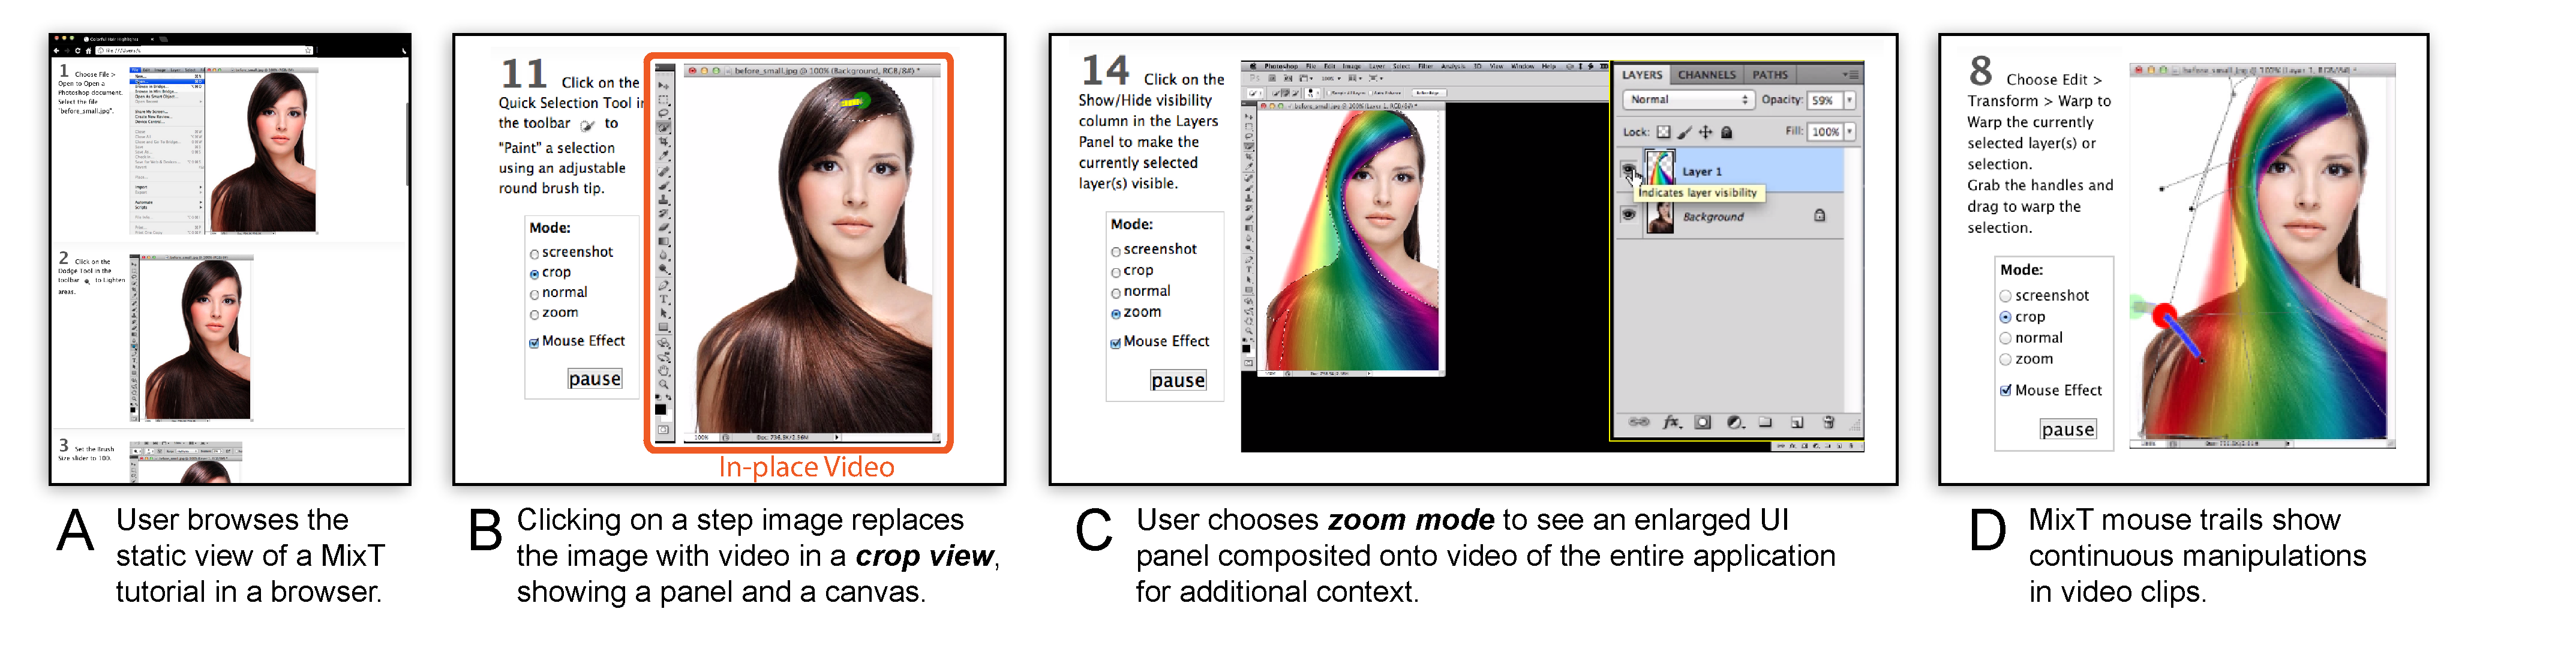
\includegraphics[width=\textwidth]{\intro/fig/mixt}
  \caption{MixT generates tutorials that contain static and video information from task demonstrations. Videos are automatically edited and offer different views to highlight the most relevant screen areas for a step. Visualizing mouse movement helps user understand a complex action.}
  \label{fig:mixt_intro}
\end{figure*}

% ----- DemoWiz ----- %

MixT offers a novel way of navigating structural content with a combination of static and video presentations. An additional effort is to help viewers expect \emph{when} and \emph{what} action is coming next while a video is playing. I design \emph{DemoWiz}, a system that augments a screencast video with visualizations (Figure~\ref{fig:demowiz_intro}). By logging the input events of a software demonstration, DemoWiz overlays glyphs to guide viewers to the next action along with the time remaining before the action occurs. This enables followers to anticipate the video content rather than react to it.
%
My study showed that fewer anticipation errors and delays were made with DemoWiz.

\begin{figure*}[t]
\centering
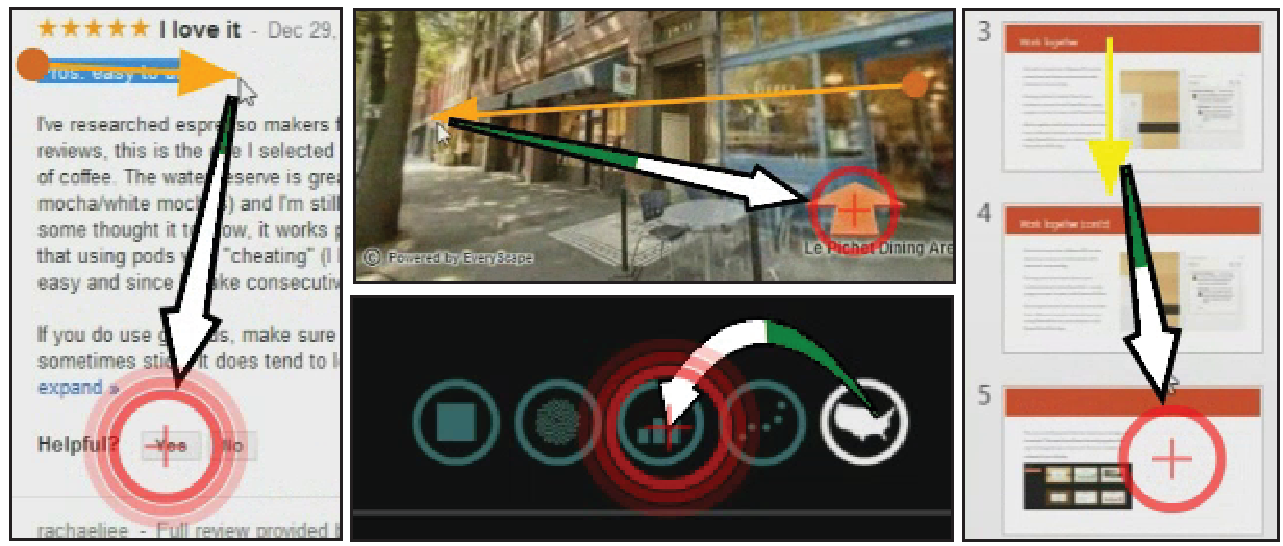
\includegraphics[width=0.6\columnwidth]{\intro/fig/DemoWiz}
\caption{DemoWiz visualizes input events in a screencast video to help viewers anticipate the upcoming event for narrating a software demonstration in a live presentation.}
\label{fig:demowiz_intro}
\end{figure*}

\subsection{Tutorial Generation from Software Demonstration}

While new tutorial formats are shown to be useful, manually creating instructions can be extremely time- and effort-consuming. In response, I design computational methods to automate the creation process from an author demonstration. MixT and DemoWiz capture screencast video and input device events from a walk-through of a software application. MixT also traces application commands for analysis. Computer vision and visualization techniques are integrated to segment a video into steps, extract salient information, and add visual highlights.
%
In addition, DemoWiz supports the editing phase where authors can adjust the timing of events in a video. Playback speed of recorded actions can be adjusted or skipped via a lightweight editing UI. My studies showed that our algorithms for step segmentation, event detection, and visualization were effective (\textless8\% error rate in MixT and 0\% in DemoWiz).

\subsection{Interactive Tutorial Authoring from Physical Demonstration}

% ----- DemoCut ----- %

Moving beyond software applications, I found it interesting yet challenging to design systems for everyday tasks that take place in the physical world, where activity recognition remains an open research question.
%
Specifically, I focus on Do it yourself (DIY) projects, which help people learn knowledge and skills to complete building or repairing work independently.

I developed \emph{DemoCut}, a semi-automatic video editing system that improves the quality of amateur instructional videos for physical tasks (Figure~\ref{fig:democut_intro}). DemoCut asks users to describe key ``moments'' in a recorded demonstration video using a set of markers. Based on the annotations, my system analyzes the audio and visual activities to automatically organize the video into meaningful segments. Editing decisions are applied to support both \emph{temporal effects} that increase playback speed or skip segments, as well as \emph{visual effects}, such as zooming, subtitles, and visual highlights. A playback interface allows users to quickly review and edit the automatically generated effects.
%
Video tutorials created by DemoCut in five DIY domains were concise in terms of video length and descriptive instructions with low effect error rates. In most cases, DemoCut successfully identified segments where the ``Fast Motion'' or ``Skip'' effects condensed the tutorial.

% \emph{DemoCut} segments a video recording of a physical demonstration (e.g., a long cooking process) based on user annotations and video and audio analysis (Figure~\ref{fig:democut_intro}). It automatically applies video editing effects (e.g., skip, speedup, and zoom) to create concise instructions. A playback interface enables lightweight editing for authors to review the results.

\begin{figure*}[t]
  \centering
  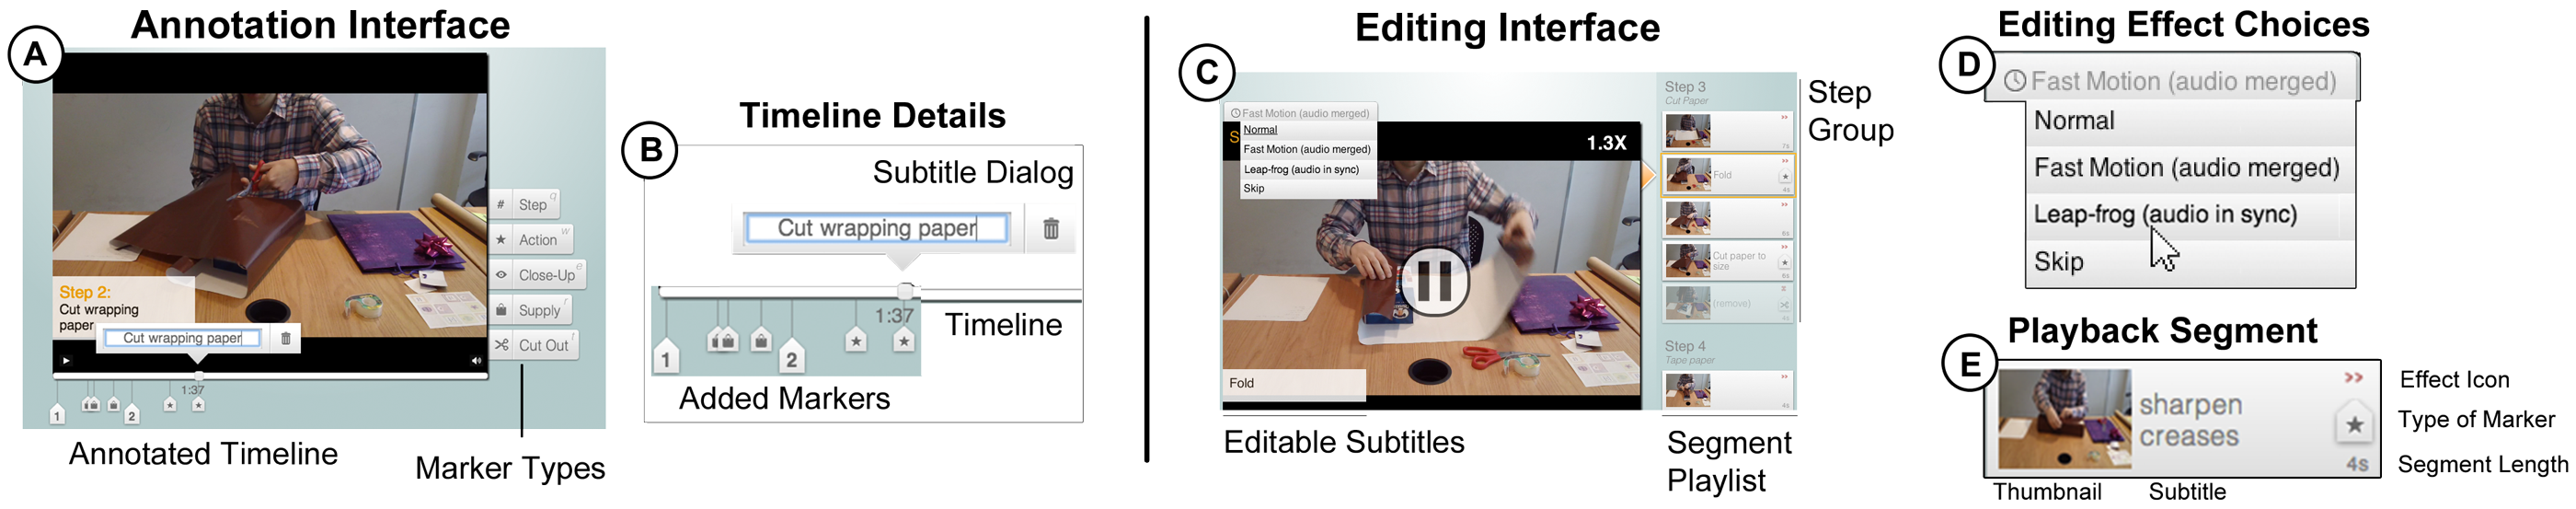
\includegraphics[width=\textwidth]{\intro/fig/DemoCut}
  \caption{DemoCut asks users to mark key moments in a recorded video of demonstration using a set of marker types (Left). Based on these markers, the system uses audio and video analysis to automatically organize the video into meaningful segments and apply appropriate video editing effects. A playback UI provides lightweight editing for authors to review and modify automatic results (Right).}
  \label{fig:democut_intro}
\end{figure*}

% ----- Kinectograph ----- %
Through the process of designing DemoCut for automatic DIY video editing, I observed that for tasks that require larger space and more movements, instructors often have to adjust the position and viewing angle of a camcorder. More advanced authors would set up multiple cameras and later select the best shot from video streams.
%
To enable authors to focus on their demonstration during the recording phase, I design \emph{Kinectograph}, a filming device that automatically tracks and follows specific body parts, e.g., hands, of an instructor in a video (see Figure~\ref{fig:kinectograph_intro}). It utilizes a Kinect depth sensor to track skeletal data and adjusts the camera angle via a 2D pan-tilt gimbal mount. Authors can freely move around in space to demonstrate a task and monitor real-time video preview through a tablet application.

\begin{figure}[!t]
  \centering
  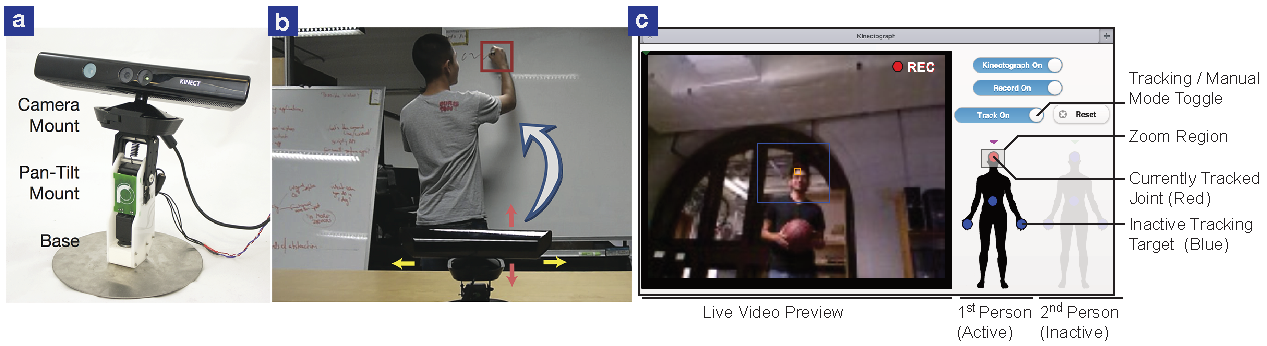
\includegraphics[width=\columnwidth]{\intro/fig/KinectographUI}
  \caption{(a) Kinectograph is composed of a Kinect camera to track user movement and a motorized dock to pan and tilt the camera so that the user (or their hand) remains centered in the recorded video. (b) Here the device follows the users' hand while he is illustrating. (c) A mobile control UI enables presenters to preview and control in real-time. \tofix{Keep the label style consistent}}
\label{fig:kinectograph_intro}
\end{figure}

% ----- DemoDraw ----- %

The successful experiences supporting software and DIY tutorials motivated me to apply my demonstration-based approach to a domain that is entirely driven by motions. For sign language, dance, and gesture-based games, instructors aim to present physical activities in a concise way for learners to follow. Using illustrations with visual highlights, human motions can be delivered in time and space as a diagram. However, current practices require authors to manually sketch or trace subjects from photographs, which is time-consuming and difficult to make changes once created.

I design \emph{DemoDraw}, a system that generates concise illustrations from user demonstration (see Figure~\ref{fig:demodraw_intro}). With DemoDraw, a user records one or more motions by physically demonstrating in front of a Kinect sensor. DemoDraw captures the RGB-D information and logs the location and orientation data of user's whole body in a 3D space. It then maps the data to a 3D humanoid avatar and applies Non-Photorealistic Rendering (NPR) effect to create line illustrations. Based on user's speech labels and motion analysis, DemoDraw renders motion arrows and overlays the annotations on top of the model to generate step-by-step illustrative diagrams.

\begin{figure}[t]
  \centering
  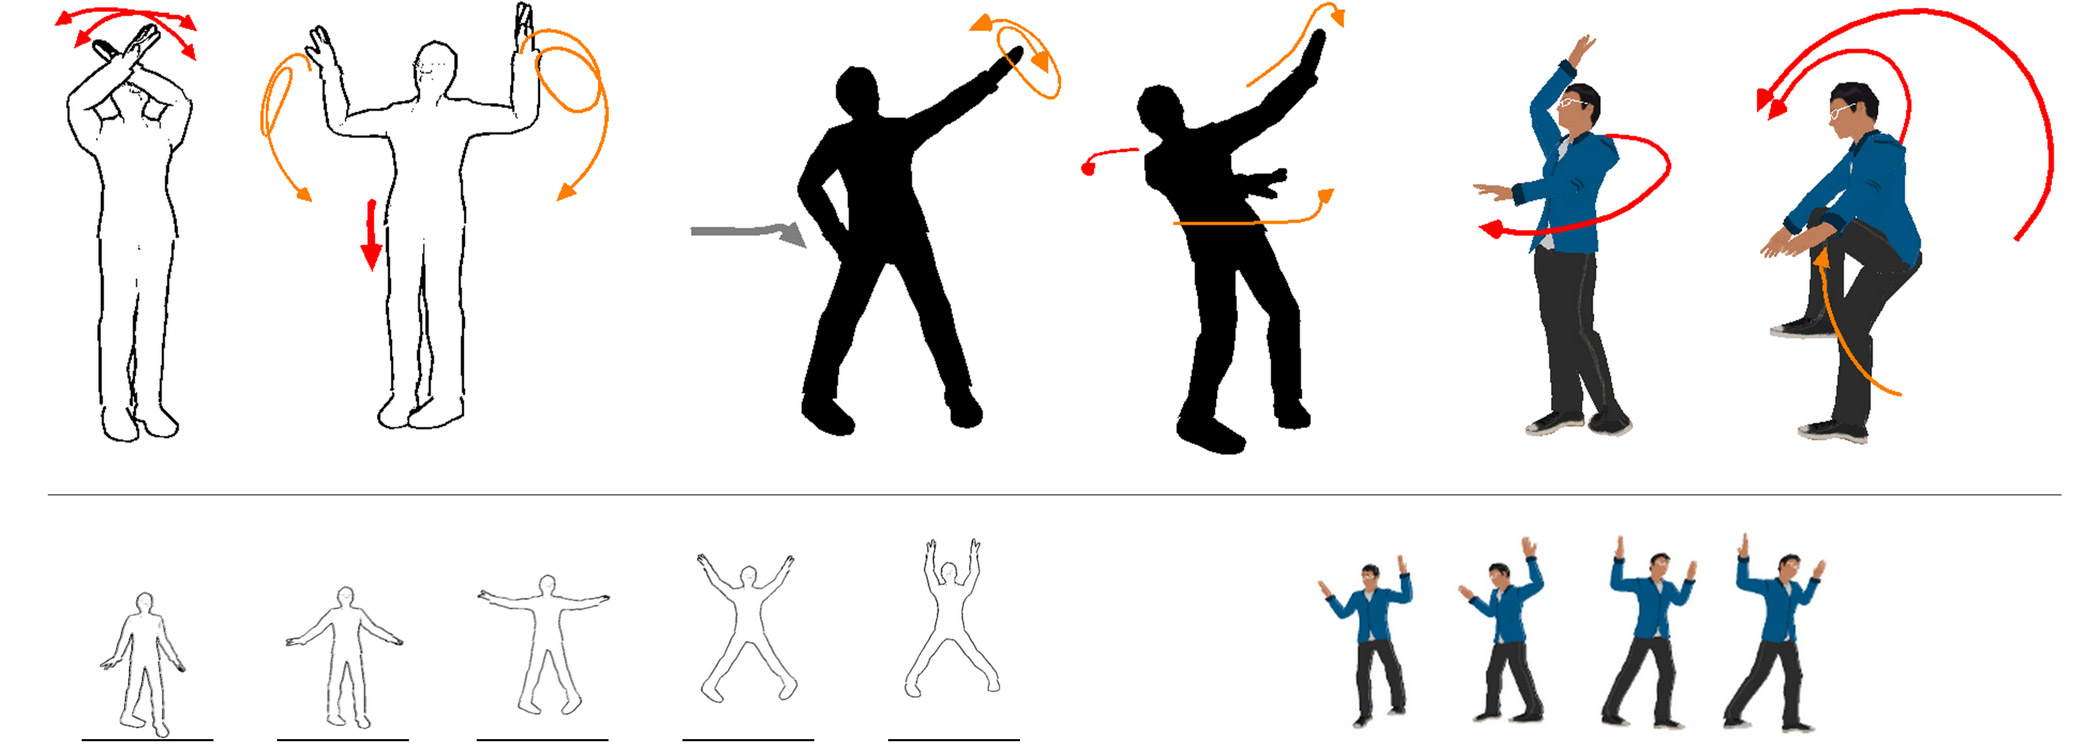
\includegraphics[width=\columnwidth]{\intro/fig/DemoDraw}
  \caption{DemoDraw: (a) multi-modal ``Demonstration Interface'' to capture motion, verify results, and re-perform portions if needed; (b) conventional Refinement Interface for refinement and exploring other visualization styles; (c-d) examples of illustration styles. \tofix{Keep the label style consistent}}
  \label{fig:demodraw_intro}
\end{figure}

% ---------------------------------------------------------------

\section{Thesis Contributions}

Overall, my video-based approaches consider key events or moments that are important to a learner. This information can be derived from software event logs or human annotation of physical tasks when automatic recognition remains challenging. Based on the metadata and video streams, I propose automatic methods to generate concise instructions for two task domains, software applications and physical tasks (see Figure~\ref{fig:space}). I demonstrate a series of systems that consider stages of tutorial creation and learning.
%
I present the rationale and technical challenges of these interactive system designs. Each system is evaluated both quantitatively and qualitatively to study the usability in authoring and learning. The contributions of this dissertation include:

\begin{figure}[t]
  \centering
  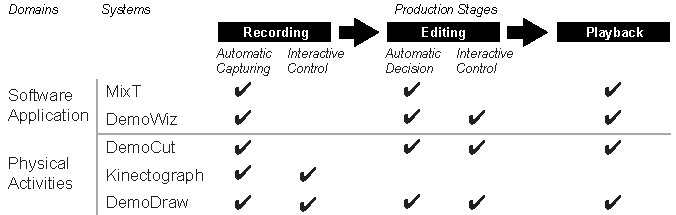
\includegraphics[width=0.8\columnwidth]{\intro/fig/space}
  \caption{A design space of the creation and consumption process for tutorials. It involves three phases of recording, editing, and playback in either software domain or a physical world. This dissertation proposes a series of systems that focus on various aspects in this design space. \tofix{Update this figure}}
  \label{fig:space}
\end{figure}

\begin{itemize}
  \setlength{\itemsep}{0pt}
\item New instructional formats that consider the learning factors from several domains, including software applications and physical activities.
\item Lightweight workflows in an easy-to-setup environment for amateur users to create effective instructions by demonstration.
\item Automatic or semi-automatic approaches using video and audio analysis that includes users in the loop to produce high-quality results.
\end{itemize}

% ---------------------------------------------------------------

\section{Overview}

The rest of my thesis is structured as follows:
%
In Chapter \ref{chapter_background}, I define terminology used in instruction creation and consumption process based on literature. I review studies on why people rely on tutorials in general, how the formats of instructions matter, and the current practices of authoring instructions.
%
In Chapter \ref{chapter_related_work}, I review the literature on research and technologies used in supporting activities of authoring and consuming instructions.

I presented two systems that support consuming tutorials for software applications.
% MixT
In Chapter \ref{chapter_mixt}, I present my study on how a new tutorial format supports learners in following step-by-step instructions with mixed media, including static text, images, and video clips. I introduce my creation tool called MixT, which automatically generates such new tutorial format from an author demonstration in a software application.

% DemoWiz
Chapter \ref{chapter_demowiz} introduces DemoWiz, a system that assists viewers in capturing the timing of input events in a screencast demo video. DemoWiz supports recording, editing, and viewing stages in a production process with an authoring and playback UI.

Then, I introduced three systems designed for real-world tasks that involve physical demonstrations.
% DemoCut
In Chapter \ref{chapter_democut}, I demonstrate a semi-automatic tool for DIY video editing. My system, called DemoCut, provides two authoring interfaces, annotation and editing, that enable users to mark a demo video and review and modify the automatically edited results. The design is based on an fundamental understanding of DIY activities.

% Kinectograph
In Chapter \ref{chapter_kinectograph}, I focus on a recording device design that automatically follows a demonstrator for filming instructional videos. The Kinectograph system tracks a user's position and body parts and provides an authoring interface for real-time control.

% DemoDraw
Finally, in Chapter \ref{chapter_demodraw}, I present a multimodal approach for users to generate motion illustrations by physically demonstrating the movements. My system, DemoDraw, segments speech and 3D joint motion captured by a Kinect RGB-D sensor into a sequence of motion segments. A series of illustrations is automatically generated using a stylistically rendered 3D avatar annotated with arrows to convey movements. Users can navigate existing illustrations using speech and amend or re-perform motions if needed. They can also edit detailed visualization parameters via an editing interface.

% Conclusion
Throughout this thesis, I discuss how my video-based approaches increase the quality of amateur-produced video instructions. Chapter 8 concludes my work on tutorial creation and consumption in both software and physical instructions. New directions for future research on interactive tutorials are proposed.

% ---------------------------------------------------------------

\section {Prior Publications}

This dissertation is based on papers published in previous ACM conference proceedings: the MixT system was published at UIST 2012 \cite{Chi:2012:MAG:2380116.2380130}; DemoWiz at CHI 2014 \cite{Chi:2014:DRS:2556288.2557254}, DemoCut at UIST 2013 \cite{Chi:2013:DGC:2501988.2502052}, and Kinectograph at CHI 2013 \cite{Cheng:2013:BCC:2468356.2468568}. DemoDraw \tofix{under submission: will update in middle June}.

While I am primary author on all publications and led the described projects, this research could not have been completed without my advisor Bj\"orn Hartmann and my collaborators that I have been fortunately to work with. Specifically, Dr. Mira Dontcheva and Dr. Wilmot Li provided valuable guidance on several projects (MixT, DemoCut, and DemoDraw); Dr. Steven M. Drucker and Dr. Bongshin Lee guided the DemoWiz project with their expertise on visualization; Dr. Daniel Vogel contributed to interaction and study design of DemoDraw. A group of students provided implementation and user study contributions, including Sally Ahn and Amanda Ren in MixT, Joyce Liu and Jason Linder in DemoCut, and Derrick Cheng in Kinectograph.

% We are all natural performers. Humans are proficient at demonstrating how to perform a task in action. However, articulating knowledge into a written or structured form can be extremely difficult. From dancing, repairing a machine, to operating software applications, it remains a challenge how everyday activities can be efficiently captured for a remote learner to understand.
